\documentclass[12pt]{article}
\usepackage{amsmath, amssymb}
\usepackage{booktabs}
\usepackage{graphicx}
\usepackage{hyperref}
\usepackage{geometry}
\geometry{margin=1in}

% ── Macros from estimation output ────────────────────────────────────────────
\input{../output/estimates/2period_estimates.txt}

\title{Progress Note: 2-Period Igami Model with Agglomeration}
\author{14.273 Mini Project}
\date{\today}

\begin{document}
\maketitle

\section{Overview}

This note documents the first extension of {igami2017} to incorporate
\textbf{innovation spillovers / agglomeration effects} in a simplified 2-period
setting. The goal is to understand whether the presence of other innovative firms
raises or lowers the incentive to adopt new technology.

\section{Model}

\subsection{State and Firm Types}

The market state at each period $t$ is $s_t = (n_o, n_b, n_n, n_{pe})$, where:
\begin{itemize}
  \item $n_o$: old incumbents (have \emph{not} adopted new technology),
  \item $n_b$: ``both'' incumbents (have adopted; produce with new tech),
  \item $n_n$: new entrants (using new technology),
  \item $n_{pe}$: potential entrants.
\end{itemize}
Active firms in the product market are those with $n_o + n_b + n_n > 0$.
``Both'' firms are multi-product: they continue to sell old-gen (at cost $c_o$)
while also selling new-gen (at cost $c_{n,t}$). This is the source of the
\textbf{cannibalization effect}: by expanding new-gen supply, a ``both'' firm
depresses the old-gen price it receives, creating a disincentive to innovate that
is absent for pure new entrants.

\subsection{Timing Within Each Period}

\begin{enumerate}
  \item \textbf{Product market:} Cournot competition in \emph{two differentiated
        markets} (old-generation and new-generation products) with linear inverse
        demand:
        \begin{align}
          P_o &= A - \frac{B}{M}\,Q_o - \frac{\rho B}{M}\,Q_n, \label{eq:demand_o}\\
          P_n &= A - \frac{B}{M}\,Q_n - \frac{\rho B}{M}\,Q_o, \label{eq:demand_n}
        \end{align}
        where $\rho \in [0,1)$ is the cross-market substitution parameter.
        Old firms ($n_o$) compete only in the old-gen market at cost $c_o$.
        New entrants ($n_n$) compete only in the new-gen market at cost $c_{n,t}$.
        ``Both'' firms ($n_b$) are \emph{multi-product}: they sell in both markets
        simultaneously and internalize the \textbf{cannibalization} effect --- their
        new-gen output reduces demand for their own old-gen product.
  \item \textbf{Private shocks:} Each firm draws i.i.d.\ cost shocks
        $\varepsilon_{i,a} \sim \mathrm{Gumbel}(0, \sigma)$ for each action $a$.
  \item \textbf{Discrete choices:}
        \begin{itemize}
          \item old: $\{\text{stay}, \text{innovate}, \text{exit}\}$
          \item both/new: $\{\text{stay}, \text{exit}\}$
          \item pe: $\{\text{enter}, \text{quit}\}$
        \end{itemize}
  \item \textbf{Transition} to period $t+1$.
\end{enumerate}

\subsection{Agglomeration Extension}

The new-technology marginal cost depends on the number of firms already using it:
\begin{equation}
  c_{n,t} = c_{n,0} - \gamma \cdot (n_{b,t} + n_{n,t}), \qquad \gamma \geq 0.
  \label{eq:agglom}
\end{equation}
When $\gamma = 0$ the model reduces to the Igami baseline. When $\gamma > 0$,
a larger innovative cluster lowers costs for all new-tech firms (knowledge
spillover / agglomeration effect).

\subsection{Value Functions and CCPs}

With private information (EVT1 shocks), each firm's optimisation is equivalent
to a single-agent problem taking others' conditional choice probabilities (CCPs)
as given. This yields closed-form logit CCPs:
\begin{equation}
  P(a \mid \tau, s) = \frac{\exp\!\bigl(\bar{V}_{a}(\tau,s)/\sigma\bigr)}
                           {\sum_{a'} \exp\!\bigl(\bar{V}_{a'}(\tau,s)/\sigma\bigr)},
\end{equation}
where $\bar{V}_a$ is the systematic utility of action $a$:
\begin{equation}
  \bar{V}_a(\tau, s) = \pi_\tau(s) + \text{cost}(a) + \beta \,
  \mathbb{E}\!\left[ V_{t+1}(\tau', s') \mid s, a_i = a,\, \mathrm{CCP}_{-i} \right].
\end{equation}

\subsection{Solution Method}

The model is solved by \textbf{backward induction} in two steps:
\begin{enumerate}
  \item \textbf{Terminal period ($t=1$):} $V_1(\tau, s_1) = \pi_\tau(s_1)$,
        where Cournot profits use the agglomeration-adjusted cost
        $c_{n,1} = c_{n,0} - \gamma(n_{b,1} + n_{n,1})$.
  \item \textbf{Period $t=0$:} For each state $s_0$, compute CCPs by iterating
        the logit fixed-point until convergence (within-period equilibrium).
        The transition distribution is computed exactly via products of
        independent Binomial/Multinomial draws.
\end{enumerate}
No cross-period iteration is required; this is a one-pass backward induction,
consistent with Igami's (2017) solution algorithm.

\section{Calibration}

The calibration is illustrative (not estimated from data) and is summarised in
Table~\ref{tab:params}.

\begin{table}[h]
  \centering
  \caption{Illustrative calibration}
  \label{tab:params}
  \begin{tabular}{clc}
    \toprule
    Parameter & Description & Value \\
    \midrule
    $A$       & Demand intercept              & 3.0  \\
    $B$       & Demand slope                  & 1.0  \\
    $M$       & Market size                   & 1.0  \\
    $c_o$     & Old-tech marginal cost        & 1.5  \\
    $c_{n,0}$ & New-tech baseline cost        & 0.5  \\
    $\beta$   & Discount factor               & 0.9  \\
    $\kappa$  & Innovation cost               & 0.3  \\
    $\phi$    & Entry cost                    & 0.2  \\
    $\sigma$  & EVT1 scale                    & 1.0  \\
    $\gamma$  & Agglomeration (comparative statics) & varied \\
    $\rho$    & Cross-market substitution     & 0.5  \\
    \bottomrule
  \end{tabular}
\end{table}

The initial state of interest is $s_0 = (n_o, n_b, n_n, n_{pe}) = (4,1,1,2)$,
loosely inspired by the early HDD market structure in Igami (2017).

\section{Results}

\subsection{Baseline vs.\ Agglomeration}

Table~\ref{tab:baseline_vs_agglom} compares equilibrium CCPs at $s_0$ for
$\gamma = 0$ (baseline) and $\gamma = \gammaAgglom$.

\begin{table}[h]
  \centering
  \caption{CCPs at $s_0 = (4,1,1,2)$: baseline vs.\ agglomeration ($\gamma = \gammaAgglom$)}
  \label{tab:baseline_vs_agglom}
  \begin{tabular}{lcc}
    \toprule
     & $\gamma = 0$ & $\gamma = \gammaAgglom$ \\
    \midrule
    $P(\text{innovate} \mid \text{old})$ & \pInnovatBaseline & \pInnovatAgglom \\
    $P(\text{enter}    \mid \text{pe})$  & \pEnterBaseline   & \pEnterAgglom   \\
    \bottomrule
  \end{tabular}
\end{table}

Agglomeration raises both the innovation and entry rates. Intuitively, a larger
innovative cluster lowers future costs for new-tech firms, increasing the expected
continuation value of innovating or entering.

\subsection{Comparative Statics in $\gamma$}

Table~\ref{tab:compstats} reports equilibrium CCPs as $\gamma$ varies from 0 to
0.30, and Figure~\ref{fig:compstats} plots the same.

\begin{table}[h]
  \centering
  \caption{CCPs vs.\ agglomeration parameter $\gamma$}
  \label{tab:compstats}
  \begin{tabular}{ccc}
\hline
$\gamma$ & $P(\text{innovate} | \text{old})$ & $P(\text{enter} | \text{pe})$ \\
\hline
0.00 & 0.3135 & 0.5061 \\
0.05 & 0.3206 & 0.5139 \\
0.10 & 0.3282 & 0.5221 \\
0.15 & 0.3314 & 0.5258 \\
0.20 & 0.3318 & 0.5263 \\
0.25 & 0.3315 & 0.5260 \\
0.30 & 0.3316 & 0.5260 \\
\hline
\end{tabular}
\end{table}

\begin{figure}[h]
  \centering
  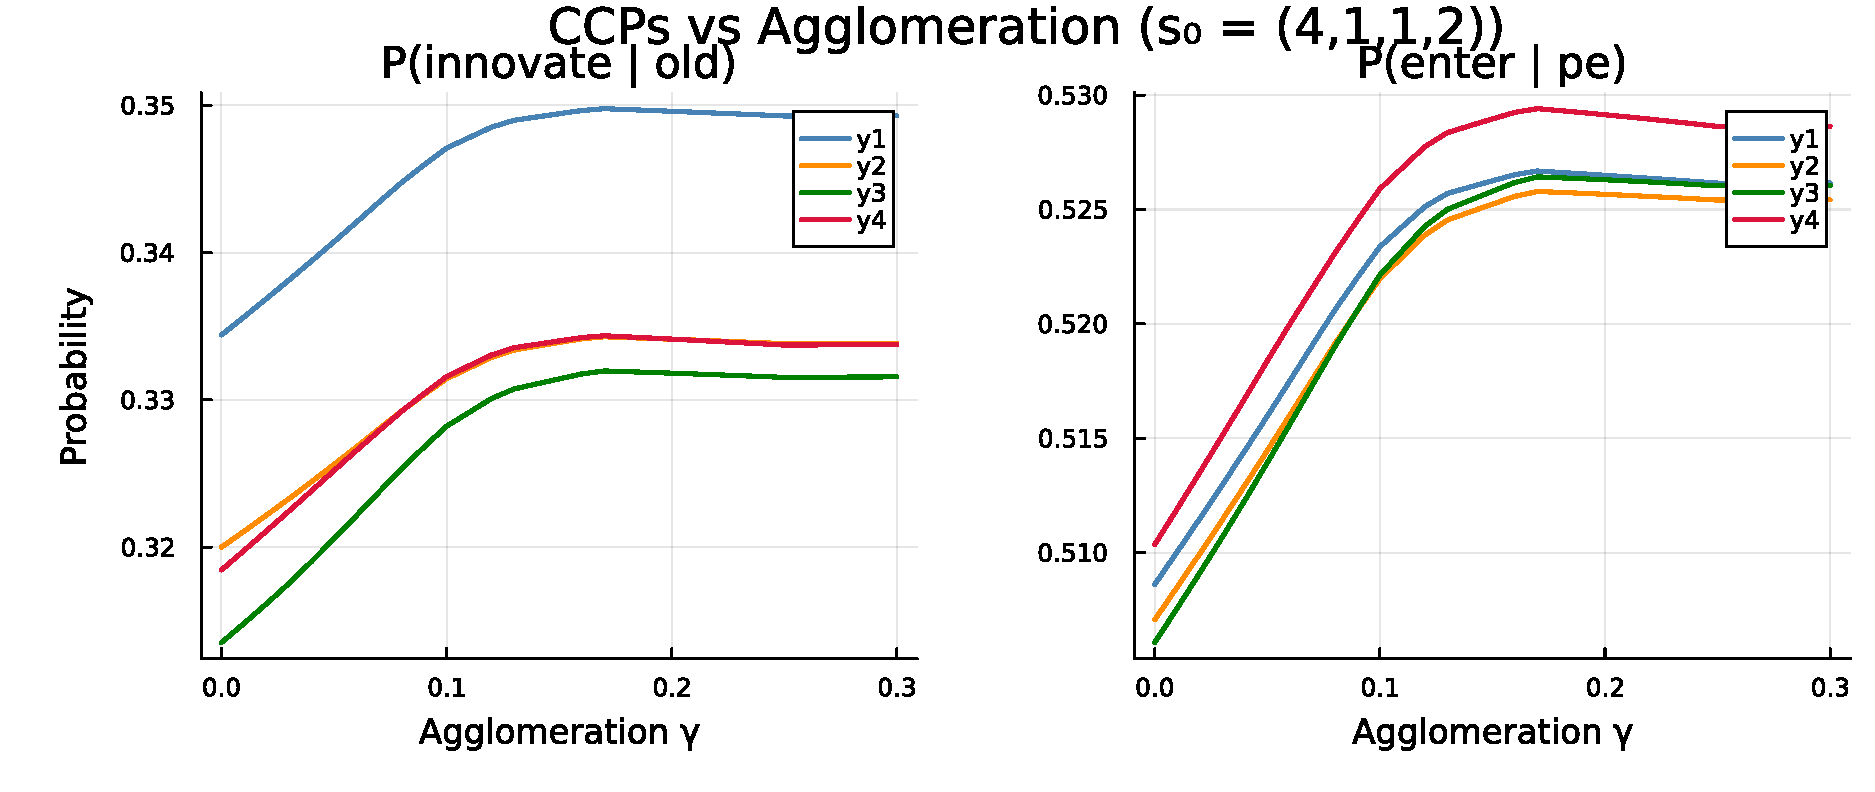
\includegraphics[width=0.7\textwidth]{../output/figures/comp_stats_agglomeration.pdf}
  \caption{$P(\text{innovate}\mid\text{old})$ and $P(\text{enter}\mid\text{pe})$
           as functions of $\gamma$ at $s_0 = (4,1,1,2)$.}
  \label{fig:compstats}
\end{figure}

\subsection{Comparative Statics in $\rho$ (Cannibalization)}

Figure~\ref{fig:cannibalization} plots equilibrium CCPs as the substitution
parameter $\rho$ varies from 0 (independent markets) to 0.95 (near-homogeneous
goods), holding $\gamma = 0.05$.

\begin{figure}[h]
  \centering
  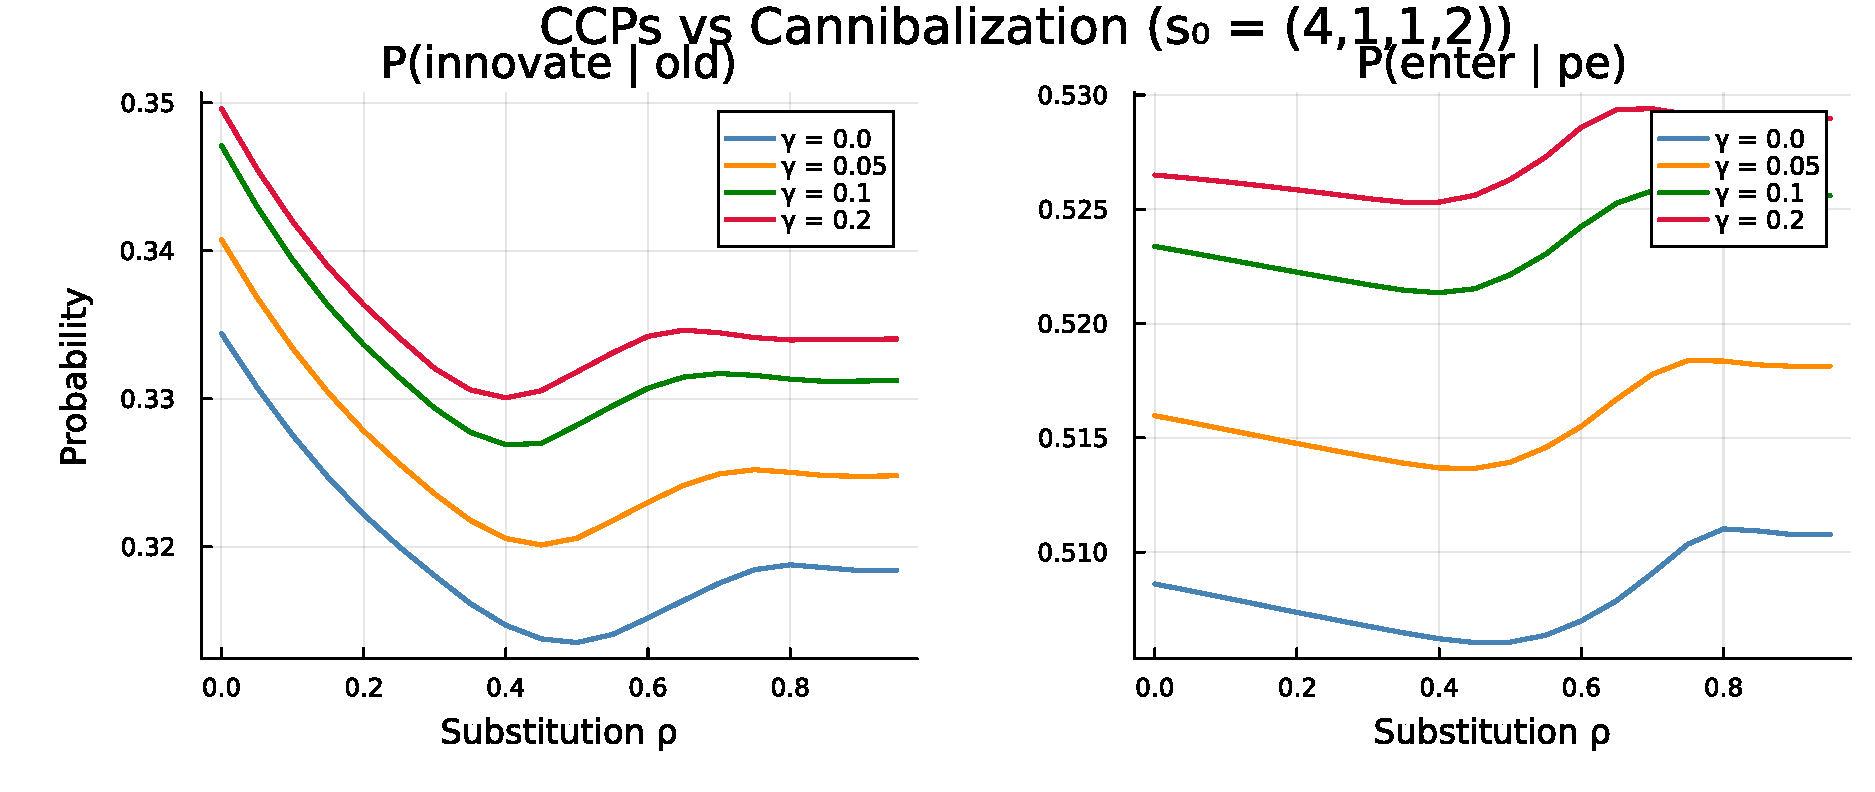
\includegraphics[width=0.7\textwidth]{../output/figures/comp_stats_cannibalization.pdf}
  \caption{$P(\text{innovate}\mid\text{old})$ and $P(\text{enter}\mid\text{pe})$
           as functions of $\rho$ at $s_0 = (4,1,1,2)$, $\gamma = 0.05$.}
  \label{fig:cannibalization}
\end{figure}

\subsection{Discussion}

Three features of the comparative statics are notable:
\begin{enumerate}
  \item \textbf{Positive agglomeration effect:} Higher $\gamma$ unambiguously
        raises the innovation rate for small values of $\gamma$. This confirms
        the model's central prediction: knowledge spillovers encourage adoption.
  \item \textbf{Cannibalization deters innovation:} Higher $\rho$ (stronger
        substitution between old-gen and new-gen) reduces the profit of ``both''
        firms by depressing old-gen prices. In the calibration, per-firm ``both''
        profit falls from $\approx 0.531$ at $\rho=0$ to $\approx 0.327$ at
        $\rho=0.5$. This is the central mechanism in Igami (2017): incumbents are
        reluctant to innovate because doing so cannibalizes their existing
        old-gen revenue.
  \item \textbf{Saturation:} The innovation rate saturates near $1/3$ for large
        $\gamma$. This is a feature of the EVT1 / logit structure: with large
        $\sigma$ relative to payoff differences, all actions approach equal
        probability. In a richer calibration (smaller $\sigma$), the effect would
        be more pronounced.
\end{enumerate}

\section{Next Steps}

\begin{enumerate}
  \item Replace the illustrative calibration with Igami's (2017) structural
        estimates (Table 3 of the paper).
  \item Extend to $T > 2$ periods (the HDD panel spans 1977--1999).
  \item Add the \textbf{spatial / geographic} version of agglomeration:
        $c_{n,t}^{(g)} = c_{n,0} - \gamma \cdot N^{\mathrm{inn}}_{g(i),t}$,
        where $g(i)$ is firm $i$'s location cluster.
  \item Study welfare and industrial policy implications (e.g., R\&D subsidies).
\end{enumerate}

\bibliographystyle{aer}
\bibliography{refs}

\end{document}
